\begin{frame}[allowframebreaks]
\frametitle{Fractionally-strided convolutions}
\begin{itemize}

\item The generator uses convolutional layers that we find called
deconvolutional layers in the source code that accompanies this paper
\cite{dcganCode}, and elsewhere, but that in the paper the authors write that
we should prefer the term ``\textit{fractionally-strided}.''  

\item The computations that comprise fractionally-strided convolutions are not
clear to us from the paper or the source code that accompanies it.  

\item We find the source code unclear because the authors implement
  fractionally-strided convolutions using library functions, the source code of
  which we run out of time to peruse.  The paper lacks detail on how to compute a
  fractionally-strided convolutions.
\end{itemize}
\end{frame}

%------------------------------------------------

\begin{frame}[allowframebreaks]
\frametitle{Fractionally-strided convolutions}
\begin{itemize} 
  \item On the other hand, the github project \cite{dcganCode}
  that accompanies the paper \cite{repLearnDcgan} links to a Tensorflow
  implementation of the same code: \cite{dcganTf} where the author of this code
  implements fractionally-strided convolutions using Tensorflow's
  conv2d\_transpose.  
    
  \item We did some internet searching and found \cite{stackExConv}.
  \begin{itemize} 
    
  \item This reference plus using conv2d\_transpose in a small
      example helps us understand precisely how the fractionally-strided convolution
      operation works.  
    
      \item We feel confident to rely on conv2d\_transpose because
      the authors of the paper \cite{repLearnDcgan} we review here provide a link to
      the code in \cite{dcganTf} in their own code. 
          
      \item We feel the authors of the DCGAN's paper's endorsement of the
      Tensorflow code means conv2d\_transpose is a valid method for doing what the
      authors of \cite{repLearnDcgan} refer to as fractionally-strided convolutions,
      and that a good understanding of conv2d\_transpose is a good understanding of
      fractionally-strided convolutions.  
   \end{itemize} 
\end{itemize}
\end{frame}

%------------------------------------------------

\begin{frame}[allowframebreaks]
\frametitle{Fractionally-strided convolutions}
\framesubtitle{Diagram from StackExchange \cite{stackExConv}}
We found some example code, and a great diagram from a StackExchange.com discussion 
\cite{stackExConv}. That explains in detail how conv2d\_transpose works.
This is the diagram we found:

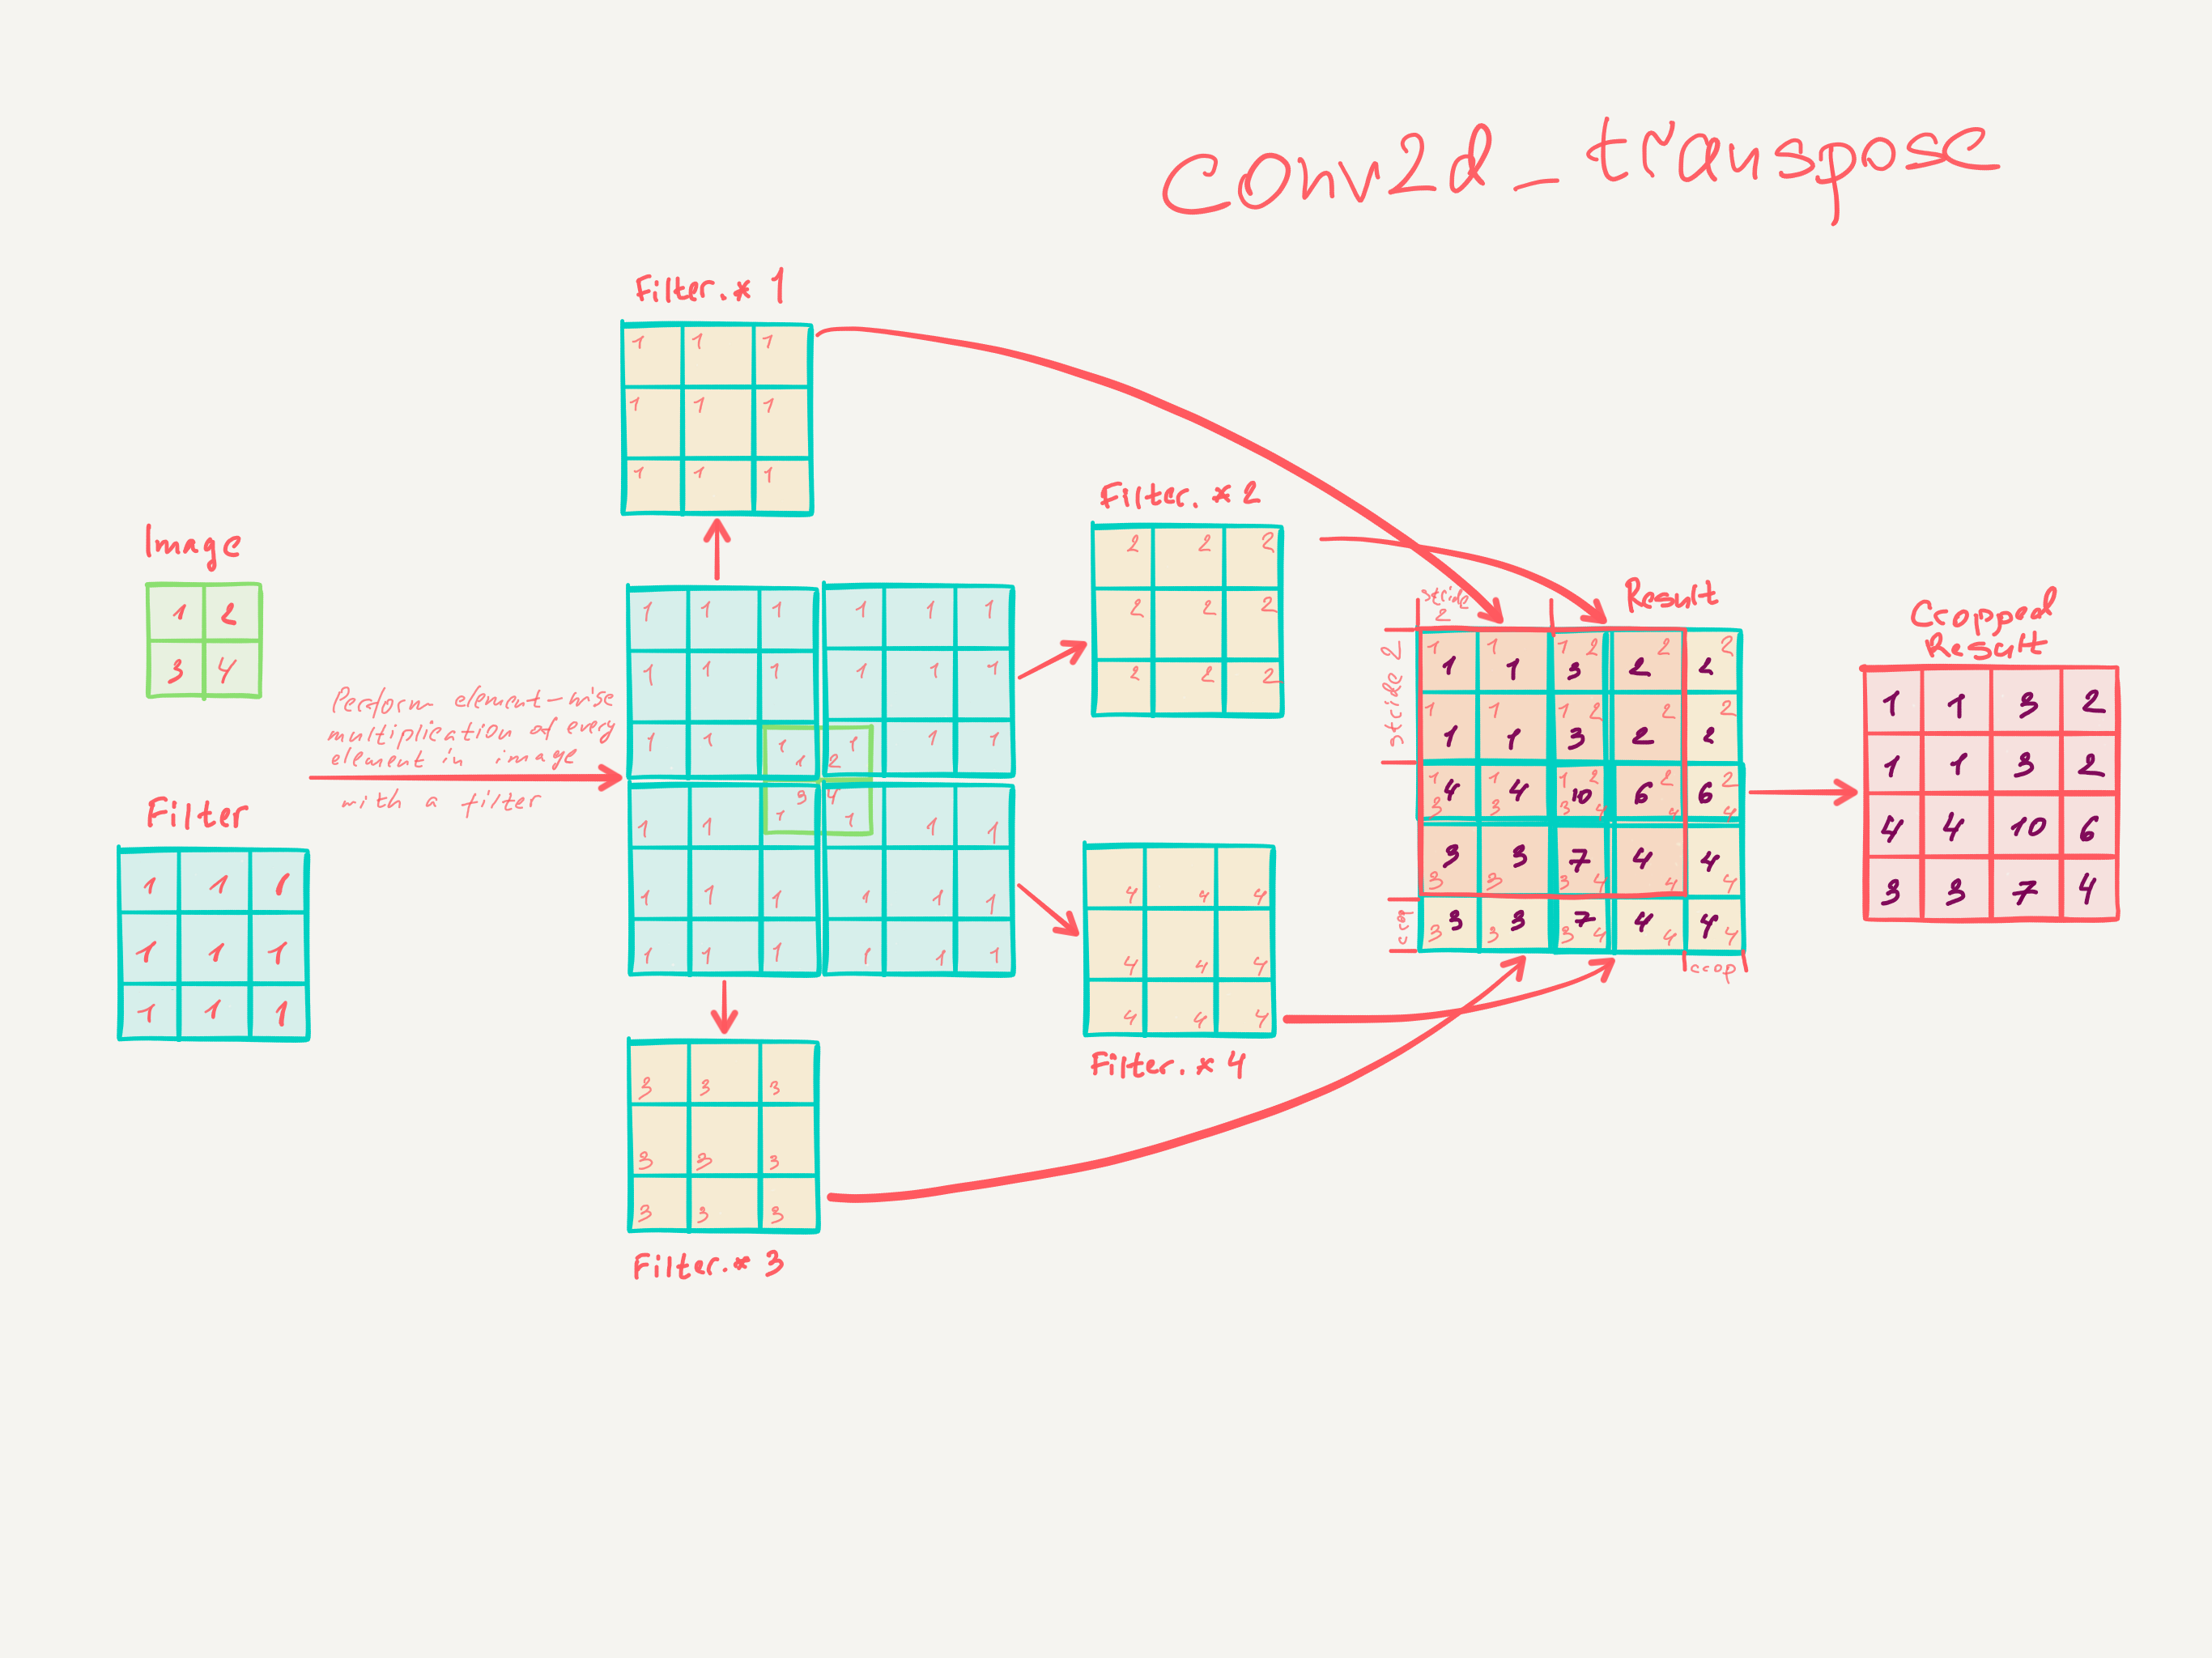
\includegraphics[scale=0.25] {conv2d_transpose-example}

\end{frame}

%-----------------------------------------------
\begin{frame}[allowframebreaks]
\frametitle{Fractionally-strided convolutions}
\begin{itemize}
\item Since anyone might write anything in online discussion forums, we decided to 
confirm that Tensorflow's conv2d\_transpose operation works as the digram implies.
conv2d\_transpose has three important parameters: input tensor, 
filter, and stride. 

\item One should be careful not to confuse the term filter we
have for conv2d\_transpose and the filters that the authors of the DCGAn's paper
show on page 9. 

\item In the context of the DCGAN paper it is better to think of the filter
parameter of conv2d\_transpose  as a kernel for the conv2d\_transpose operation,
and the filter is the result of applying conv2d\_transpose to the input tensor. 
\end{itemize}
\end{frame}

%------------------------------------------------

\begin{frame}[allowframebreaks]
\frametitle{Fractionally-strided convolutions}
\begin{itemize}

\item The next slide shows  a 4x4  input tensor, and the result of applying 
conv2d\_transpose to that tensor, with stride of 1,4,4,1. 

\item Conv2d\_transpose operates on 4 dimensional tensors, so we must embed the  4x4
matrix in a 4-dimensional tensor, and stride through it accordingly. Note on the 
next slide how most entries in the output tensor are copies of entries in the input
tensor, except where the 5x5 kernels must overlap in order to achieve the 
16x16 output.
\end{itemize}
\end{frame}

%------------------------------------------------

\begin{frame}[allowframebreaks]
\frametitle{Fractionally-strided convolutions}
The input tensor:
\[
\begin{bmatrix}
  1 & 2 & 3 & 4 \\
  5 & 6 & 7 & 8 \\ 
  9 & 10 & 11 & 12 \\
  13 & 14 & 15 & 16
\end{bmatrix}
\]
The output we can see the entries in the input matrix copied into 5x5 intermediate
tensors and then added according to the stride of 4, and values are added when
we have overlap.  We show a screen shot to prove the code runs.

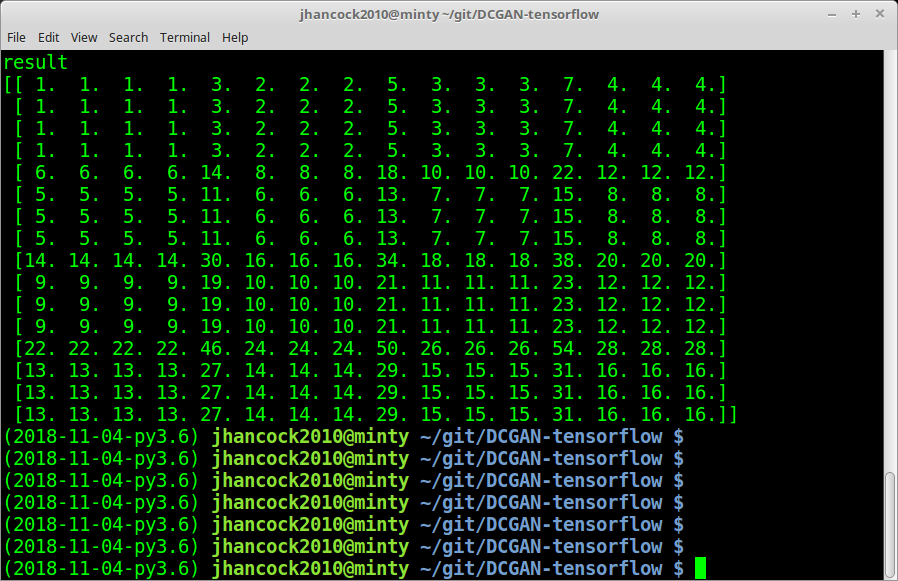
\includegraphics[scale=0.25]{conv2d-result}

\end{frame}

%------------------------------------------------

\begin{frame}[allowframebreaks]
\frametitle{Fractionally-strided convolutions}

\end{frame}


